\begin{figure}[p]
\centering
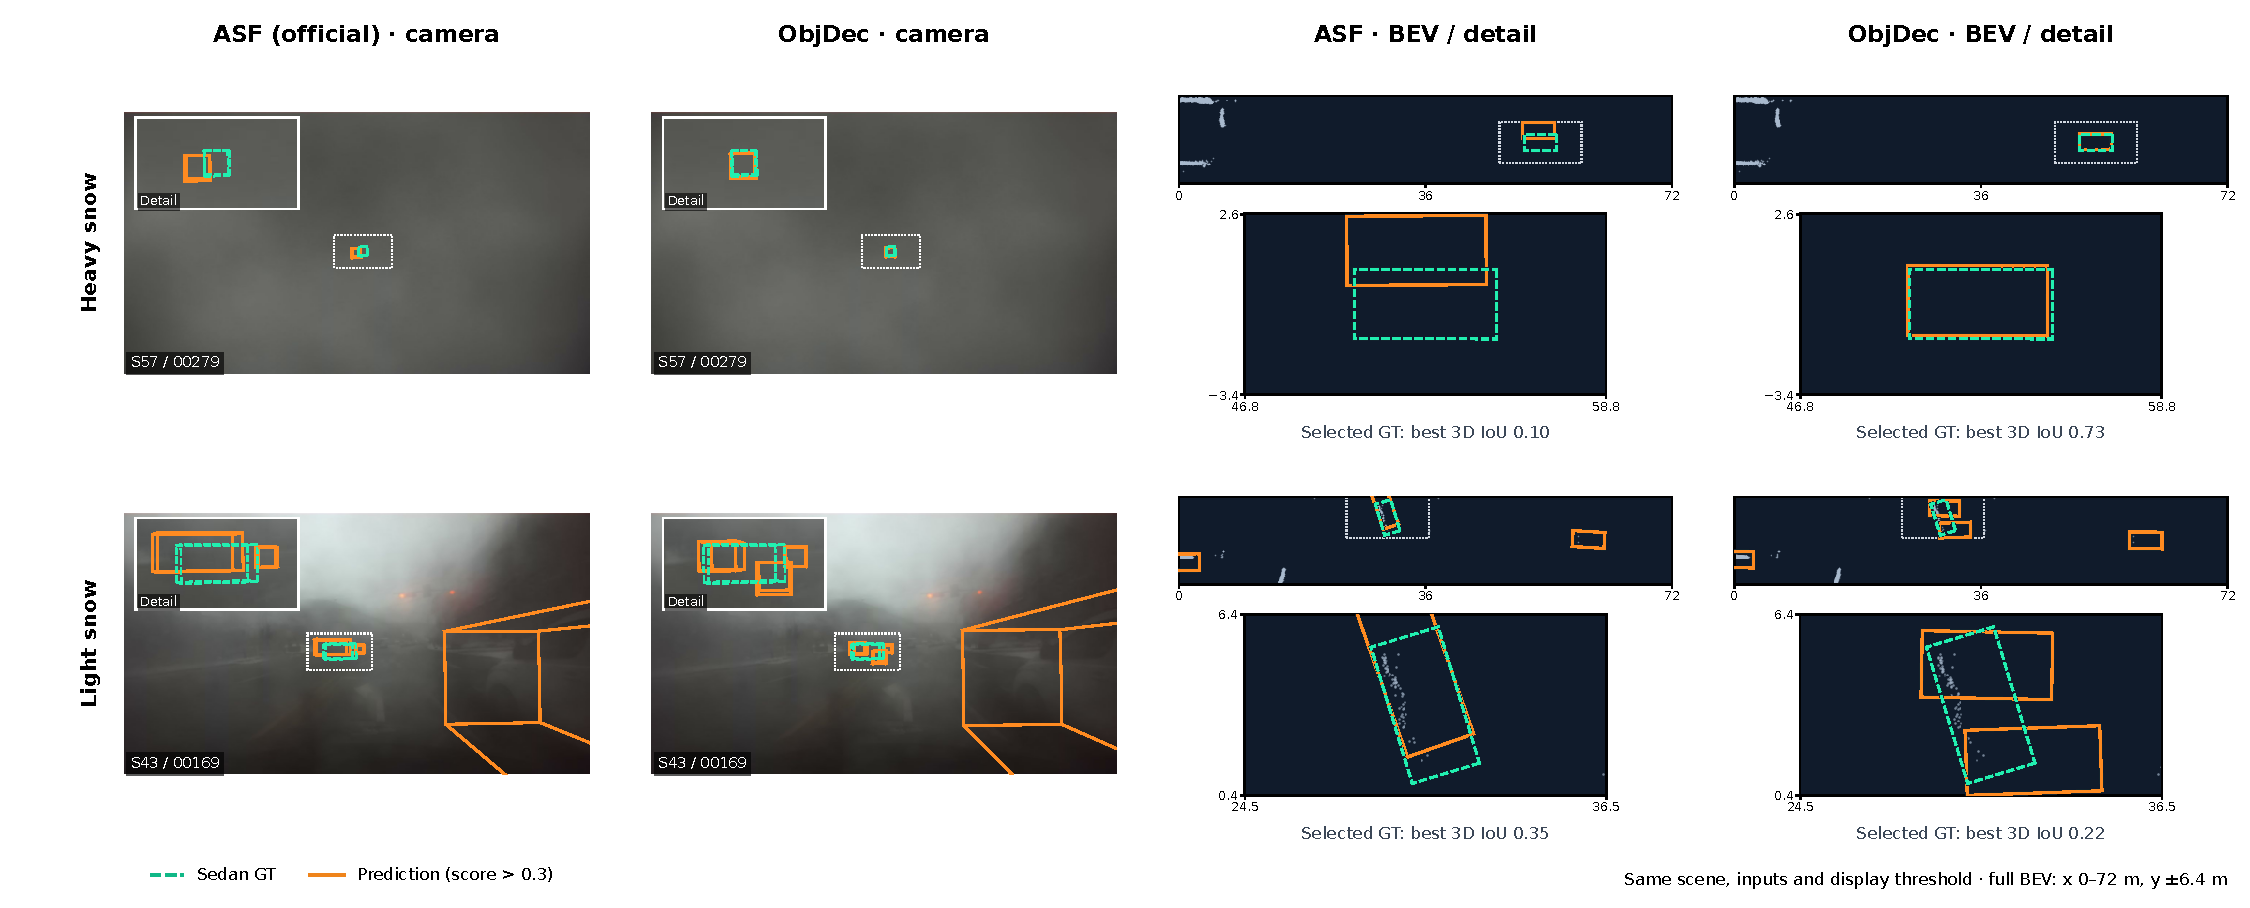
\includegraphics[width=\linewidth,height=.69\textheight,keepaspectratio]{assets/snow_counterexample.pdf}
\caption{Additional paired detections from the released ASF checkpoint and ObjDec. Green dashed boxes are GT and orange solid boxes are predictions with score>0.3; both methods use identical camera projections and detail windows. The selected heavy-snow object's maximum geometric 3D IoU increases from 0.095 to 0.728, whereas the light-snow object's decreases from 0.354 to 0.223. The latter also appears in the seven-weather appendix gate visualization, where locally high foreground response coexists with poorer localization. Foreground-related activation does not replace final box regression. Displayed IoUs describe selected-object overlap rather than AP.}
\label{fig:e3}
\end{figure}
